\begin{slide}{Motivation of Soot Attributes}
\begin{itemize}
\item Java bytecode is a relatively high-level representation
\item Lower-level optimizations, such as register allocation and bounds 
      check elemination, cannot be performed at bytecode level 
\item Some analysis results and off-line profiling information need to
      be annotated in the class file
\item Soot provides a framework to support the embedding of custom, 
      user-defined attributes in class files
\end{itemize}
\end{slide}

\begin{slide}{Java class file attributes}
\begin{itemize}
\item Attributes of {\em class\_info}, {\em method\_info}, 
      {\em field\_info}, and {\em Code\_attribute} structures
\item In fact: Code is an attribute of a method
\item Standard attributes: SourceFile, ConstantValue, Exceptions,
      LineNumberTable, LocalVariableTable
\end{itemize}
\end{slide}

\begin{slide}{Attribute format}
\small{
\begin{verbatim}
attribute_info {
  u2 attribute_name_index;
  u4 attribute_length;
  u1 info[attribute_length];
}
\end{verbatim}
}
\begin{itemize}
\item {\tt attribute\_name\_index}, the index of the attribute's name in the class files' {\em Constant Pool}
\item {\tt attribute\_length}, the length of the arrtibute's data
\item {\tt info}, an array of raw attribute data
\end{itemize}
\end{slide}

\begin{slide}{Attribute and Soot (overview)}
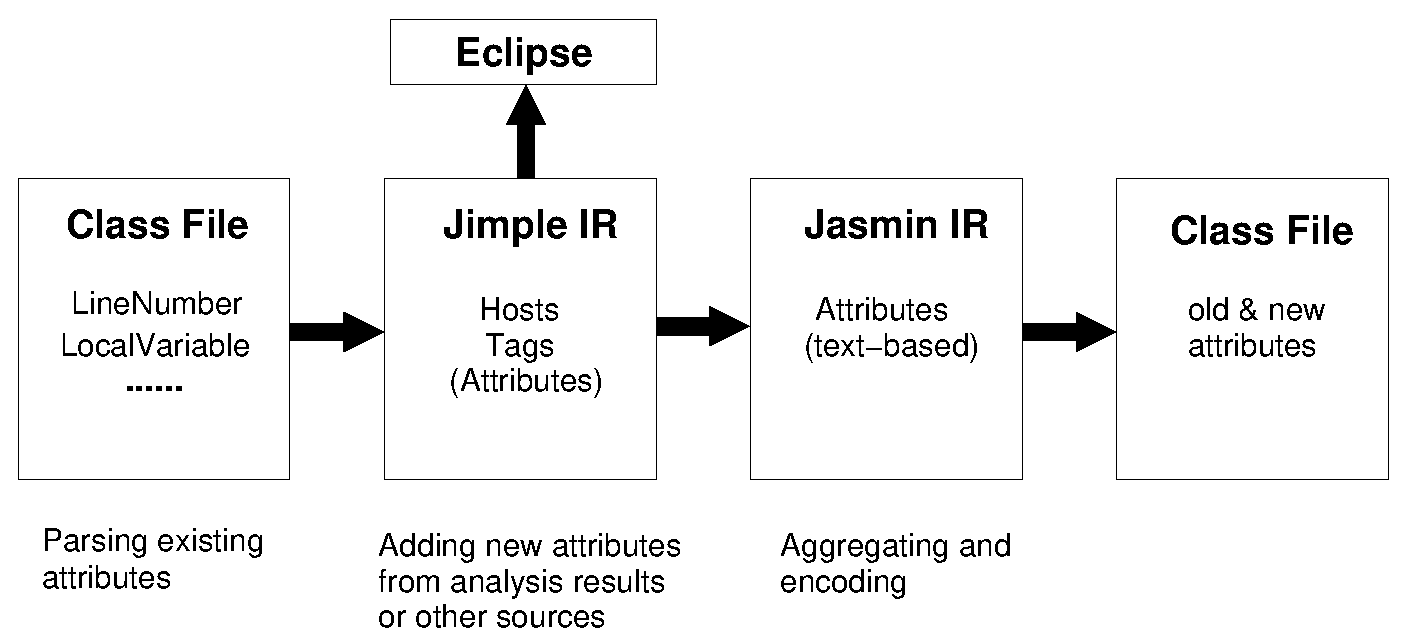
\epsfig{file=soot-attribute.eps,width=4.3in}
\begin{itemize}
\item Soot parses several standard attributes 
\item New attributes can be created and attached to Hosts
\item Users have options to design their own attribute's format
\end{itemize}
\end{slide}

%% a picture shows mapping between soot internal objects to class file structures
\begin{slide}{Tags in Soot Internals}
{\bf picture here}
\end{slide}

\begin{slide}{Hosts}
{\red Host}s are objects that can hold {\red Tag}s:
{\small
\begin{verbatim}
package soot.tagkit;
public interface Host {
  public void addTag (Tag t); 
  public Tag getTag (String aName); 
  public List getTags ();
  public void removeTag (String name); 
  public boolean hasTag (String aName); 
}   
\end{verbatim}
}
Implementations:\\
\quad {\small SootClass, SootField, SootMethod, Body} and {\small ValueBox}
\end{slide}

\begin{slide}{Tags}
{\red Tag}s are objects that can be attached to {\red Host}s:
\small{
\begin{verbatim}
package soot.tagkit;
public interface Tag {
  public String getName ();  
  public byte[] getValue () 
    throws AttributeValueException; 
}
\end{verbatim}
}
\begin{itemize}
\item {\red Attribute} attached to class file structures (class, field, method)
\item Generic tags attached to {\em ValueBox}es
\end{itemize}
\end{slide}



\begin{slide}{Tags in Soot}
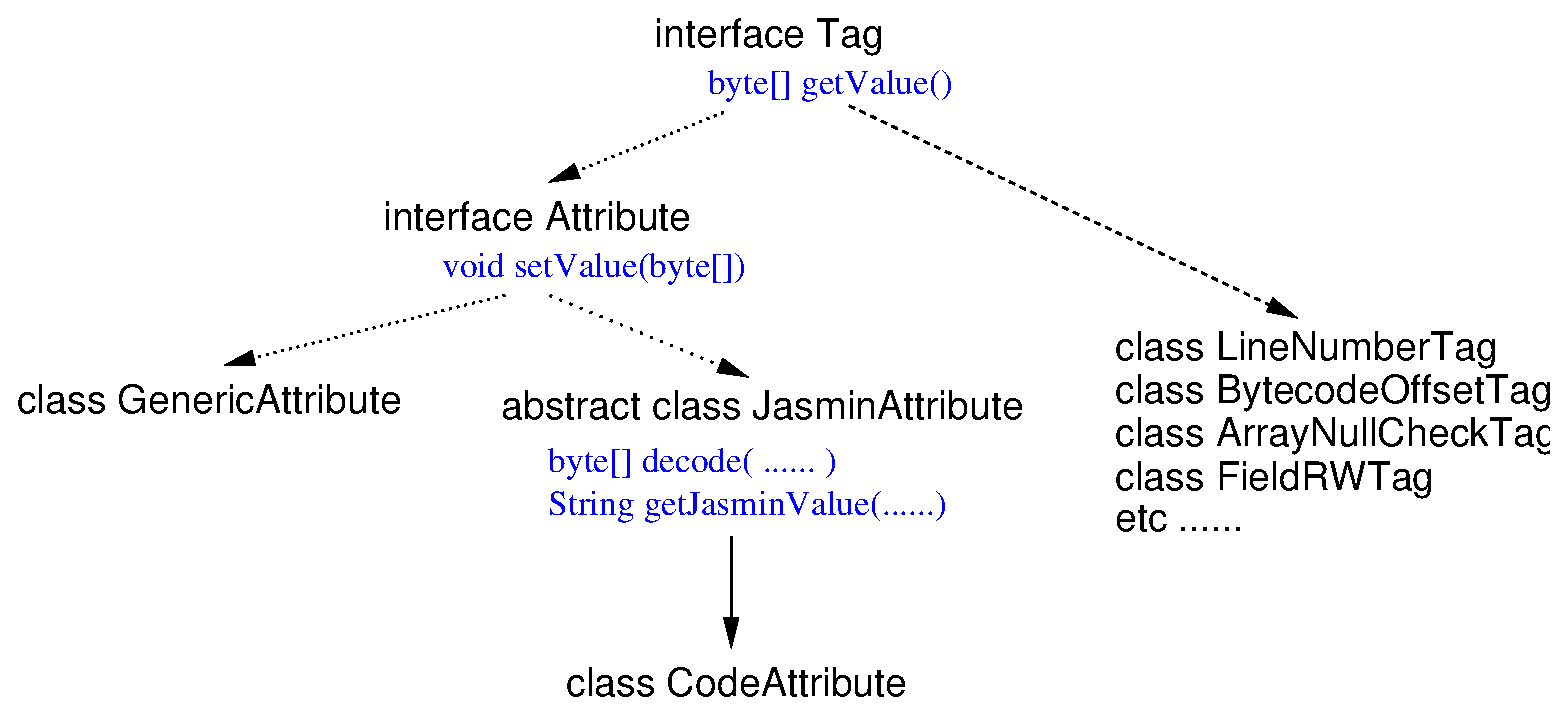
\epsfig{file=tag-hierarchy.eps, width=4.2in}
\end{slide}

%% how does soot produce tags and attributes in class file
\begin{slide}{From Soot Tags to Class File Attributes}
{\bf diagram here}
\end{slide}


\begin{slide}{Special case: attributes of Code\_attribute}
\begin{itemize}
\item Tags are attached to units, mapped into a table of (pc, value) pairs
      in class file
\item {\red TagAggregator} collects (Unit, Tag) pairs from JimpleBody, and
      produces an aggregated tag 
\item {\tt JasminAttribute} can be attached to Body
\item Soot has a default implementation: {\tt CodeAttribute}
\end{itemize}
\end{slide}

\begin{slide}{TagAggregator}
{\small
\begin{verbatim}
public abstract class TagAggregator 
  extends BodyTransformer {
  ......
  abstract boolean wantTag(Tag t);
  abstract void considerTag(Tag t, Unit u);
  abstract String aggregatedName();
  void internalTransform(Body b, ... ) { 
    ...... 
  }
}
\end{verbatim}
}
\end{slide}

\begin{slide}{Todo list for creating new attributes}
\begin{itemize}
\item Create a new Tag class, decide which structure is the host
\item If the tag is for Units, write a tag aggregator by extending {\em TagAggregator}
\item Parse attributes in bytecode consumer
\end{itemize}
\end{slide}

\begin{slide}{Example: nullness attribute}
Step 1: create NullCheckTag
\footnotesize{
\begin{verbatim}
package soot.jimple.toolkits.annotation.tags;
class NullCheckTag implements OneByteCodeTag {
  private static String NANE =''NullCheckTag'';
  private byte value = 0;
  public NullCheckTag(boolean needCheck) {
    if (needCheck) value = 0x04;
  }
  public byte[] getValue() { ... };
  ......
}
\end{verbatim}
}
\end{slide}

\begin{slide}{Example: nullness attribute}
Step 2: attach tags to units after analysis \\
{\small soot.jimple.toolkits.annotation.nullcheck.NullPointerChecker}
\footnotesize{
\begin{verbatim}
int vInfo = analysis.anyRefInfo(obj, beforeSet);
boolean needCheck = (vInfo != analysis.kNonNull); 
s.addTag(new NullCheckTag(needCheck));
\end{verbatim}
}
\end{slide}

\begin{slide}{Example: nullness attribute}
Step 3: create a tag aggregator, NullTagAggregator, and
register it in ``{\em tag}'' pack with soot.PackManager
{\scriptsize \verb$ p.add(new Transform(``tag.null'',$
   \verb$         NullTagAggergator.v())); $}

\scriptsize{
\begin{verbatim}
class NullTagAggregator extends TagAggregator {
  public boolean watTag(Tag t) {
    return (t instanceof NullCheckTag);
  }
  public void considerTag(Tag t, Unit t) {
    if ( ... ) return; // verify unit requires null check
    super.units.add( u );
    super.tags.add ( t );
  }
}
\end{verbatim}
}
\end{slide}

\begin{slide}{Control attributes format}
\begin{itemize}
\item Attributes of class, field and method provide raw data 
      via {\em byte[] getValue()} method
\item Attributes of Code\_attribute extends {\em JasminAttribute}
      which generates textual representation of (label, value)
      pairs:\\
\footnotesize{\verb$ String getJasminValue(Map instToLabel); $} \\
e.g. "NullCheckAttribute":
\footnotesize{
\begin{verbatim}
null_check_attribute {
  u2 attribute_name_index;
  u4 attribute_length;
  { u2 pc;
      u1 data;
  } [attribute_length/3];
}
\end{verbatim}
}
\end{itemize}
\end{slide}
